%%%%%%%%%%%%%%%%%%%%%%%%%%%%%%%%%%%%%%%%%%%%%%%%%%
%%%%%%%%%%%%%%%%%%%%%%%%%%%%%%%%%%%%%%%%%%%%%%%%%%
%%
%% Based one the "beamer-greek-two" template provided
%% by the Labo/
%% Adapted by Fabian Gröger, June 2020
%%
%%%%%%%%%%%%%%%%%%%%%%%%%%%%%%%%%%%%%%%%%%%%%%%%%%
%%%%%%%%%%%%%%%%%%%%%%%%%%%%%%%%%%%%%%%%%%%%%%%%%%
%%
\PassOptionsToPackage{unicode}{hyperref}
\PassOptionsToPackage{naturalnames}{hyperref}

% to use normal slides ratio
%\documentclass{beamer}

% to use 16:9 ratio
\documentclass[aspectratio=169, professionalfonts]{beamer}

%\usepackage{babel}
%\usepackage[utf8]{inputenc}


%%% FONT SELECTION %%%%%%%%%%%%%%%%%
%%% sans font %%%%%%%%%%
\usepackage{kmath,kerkis}
%\usepackage[default]{gfsneohellenic}

%%% Times NR %%%%%%%%%%
%\usepackage{newtxtext,newtxmath}
%%%%%%%%%%%%%%%%%%%%%%%%%%%%%%%%%%%%

\usepackage{color}
\usepackage{amsmath}
\usepackage{amssymb}

\usepackage{pgfgantt}
\usepackage{adjustbox}

%\usepackage{media9}
\usepackage{multimedia}

\usepackage{hyperref}
\hypersetup{
    colorlinks=true,
    linkcolor=black,
    filecolor=hslu_pink,
    urlcolor=hslu_pink,
}

%% Listings Paket ------------------------------------------------------
%%% Doc: ftp://tug.ctan.org/pub/tex-archive/macros/latex/contrib/listings/listings-1.3.pdf
\usepackage{listings, ../latex-lib/listings-rust/listings-rust}

\definecolor{codegreen}{rgb}{0,0.6,0}
\definecolor{codegray}{rgb}{0.5,0.5,0.5}
\definecolor{codepurple}{rgb}{0.5,0,0.33}
\definecolor{codepurblue}{rgb}{0.16,0.0,1.0}
\definecolor{backcolour}{rgb}{1,0.94,0.70}

\lstset{
    basicstyle =\ttfamily\color{black}\small, % Standardschrift
    commentstyle=\color{codegreen},
    keywordstyle=\bfseries\color{codepurple},
    numberstyle=\tiny\color{codegray},
    stringstyle=\color{codepurblue},
    numbers = left,              % Ort der Zeilennummern
    tabsize=2,              % Groesse von Tabs
    breakatwhitespace=false,              % An Leerzeichen umbrechen
%showspaces=true,			  % Leerzeichen anzeigen
    backgroundcolor=\color{backcolour},      % % Hintergrundfarbe der Listings
    breaklines=true,
    captionpos=b,
    keepspaces=true,
    numbersep=5pt,
    showspaces=false,
    showstringspaces=false,
    showtabs=false,
}

% Code auschnitt importieren aus datei
% example:
%\mylisting{from}{to}{language}{file}{descr}{path}
\newcommand{\mylisting}[6]{
    \lstinputlisting[language=#3,
        firstnumber=#1,
        firstline=#1,
        lastline=#2,
        caption={#4, #5},
        label={implementation_listing_#4_#5}]
    {#6}
}

%% End Listings Paket ------------------------------------------------------

%% Output console ----------------------------------------------------

%example:
%\begin{codeoutput}[red]
%This is some text inside a display environment.
%\end{codeoutput}

\usepackage{verbatim}
\definecolor{outputbackground}{rgb}{0.9, 0.9, 0.9}
\newenvironment{codeoutput}[1][black]{%
    \par\noindent
    \adjustbox{margin=1ex,bgcolor=outputbackground,margin=0ex \medskipamount}%
    \bgroup
    \minipage{\dimexpr\linewidth-2ex\relax}
    \verbatim
    \ttfamily
    \color{#1} % Set text color
    }{%
    \endverbatim
    \endminipage
    \egroup
}

%% End Output console ----------------------------------------------------


% Have subfigures and captions
\usepackage{subcaption}
\usepackage{caption}

% Tikz to crate diagrams, thanks to: https://github.com/mvoelk/nn_graphics
% Start of tikz settings
\usepackage{tikz}
\usetikzlibrary{positioning,arrows.meta}
\usetikzlibrary{matrix, chains, positioning, decorations.pathreplacing, arrows}
\usetikzlibrary{shapes,arrows,positioning,calc,chains,scopes}

\usepackage{ifthen}
\usepackage{pgfplots}
\pgfplotsset{compat=1.16}
\pgfplotsset{every axis/.append style={tick label style={/pgf/number format/fixed},font=\scriptsize,ylabel near ticks,xlabel near ticks,grid=major}}

\DeclareMathOperator{\sigm}{sigm}
\newcommand{\diff}{\mathop{}\!\mathrm{d}}

% colors
\definecolor{snowymint}{HTML}{E3F8D1}
\definecolor{wepeep}{HTML}{FAD2D2}
\definecolor{portafino}{HTML}{F5EE9D}
\definecolor{plum}{HTML}{DCACEF}
\definecolor{sail}{HTML}{A3CEEE}
\definecolor{highland}{HTML}{6D885A}

\tikzstyle{signal}=[arrows={-latex},draw=black,line width=1pt,rounded corners=4pt]

\usepackage{epstopdf}
\usepackage{graphicx}
\graphicspath{{./images/}}

% to make beautiful tables
\usepackage{booktabs}

% appendix for beamer
\usepackage{appendixnumberbeamer}

% notes on beamer template
% when using notes, make sure to have a pdf viewer, which can use the notes
% for example: https://github.com/Cimbali/pympress/
\usepackage{pgfpages}
%\setbeameroption{show notes}
%\setbeameroption{show notes on second screen=right}

%% Debugging
%\usepackage{showframe}

%%
% load HSLU thesis layout
\usepackage{HSLU_Thesis_Beamer_Layout}
\setTeipelLayout{}% options: "draft" -> Watermark

\setcounter{tocdepth}{1}
%\beamertemplatenavigationsymbolsempty
\setbeamertemplate{headline}{}

%%%%%%%%%%%%%%%%%%%%%%%%%%%%%%%%%%%%%%%%%%%%%%%%%%%%%%%%%%%%
% Presentation Info %%%%%%%%%%%%%%%%%%%%%%%%%%%%%%%%%%%%%%%%
%%%%%%%%%%%%%%%%%%%%%%%%%%%%%%%%%%%%%%%%%%%%%%%%%%%%%%%%%%%%
% title
\title[PCP-Rust]{Programming Concepts \& Paradigms\\ Team-Projekt: Rust}
% author
\author[Schilter \& Preuß]{Roman Schilter \& Jan-Henrik Preuß}
% supervisor
\supervisor{Supervisor}{Marcel Baumann \& Ruedi Arnold}
% date
\presentationDate{May 31, 2024}
%%%%%%%%%%%%%%%%

\begin{document}

% typeset front slides
\typesetFrontSlides

%%%%%%%%%%%%%%%%
% Slides each section in own file to reduce clutter and conflicts:

% Some intro stuff goes here

\begin{frame}{Die Programmiersprache Rust}
    \framesubtitle{Just a 3D-Printed gun?}
    \begin{itemize}
        \item Relativ junge Programmiersprache (seit 2010)\pause
        \item Ziel: Lückenschluss zwischen Low- und High-Level sprachen\pause
        \item Mozilla unterstützt rust entwicklung, Gründung der Rust Foundation (2021)\pause
        \item Support Linux Kernel (2021) und Android (v12)
    \end{itemize}

    \note{
        C gibt es seit 1972, C++ 1972 und Java 1995 \\
        Firefox stylo \\
        Android: Blog artikel von 2022 -> zero memory safety vulnerabilities discovered in Android’s Rust code. \\
        % https://security.googleblog.com/2022/12/memory-safe-languages-in-android-13.html \\
        65\% of High \& Critical security bugs in Chrome and Android. \\
        % https://alexgaynor.net/2020/may/27/science-on-memory-unsafety-and-security/ \\
        Linus torwald on rust (2023): "We need not stagnate, try something new. No parts of the kernel depend on rust" \\
        https://www.youtube.com/watch?v=YyRVOGxRKLg
    }
\end{frame}

% Borrowing & Move-Semantik

% Example direct code, note the [fragile] annotation
\begin{frame}[fragile,t]{Zuweisung einer Ganzzahl}
    \begin{lstlisting}[language=Rust,escapechar=@,label={lst:borrowing1}]
fn main() {
    let var1 = 1;
    let var2 = var1;

    println!("Die Werte sind: {} und {}", var1, var2);
}\end{lstlisting}
    \pause
    \codeoutput{code/02-borrowing1.txt}
    \note{
        Einfache werte können direkt einer neuen variable zugewiesen werden.
        Wie dies auch in Java möglich ist.
        Beim Verlassen der \texttt{main()} wird \texttt{var1} und \texttt{var2} aufgeräumt.
    }
\end{frame}

% Example direct code, note the [fragile] annotation
\begin{frame}[fragile,t]{Zuweisung eines Strings}
    \begin{lstlisting}[
        language=Rust,escapechar=@,label={lst:borrowing2},
        linebackgroundcolor={%
        \btLstHL<1>{}% No highlighting on first slide
        \btLstHL<2>{5}% Highlight second slide
        },
    ]
fn main() {
    let var1 = String::from("hello");
    let var2 = var1;

    println!("Die Werte sind: {} und {}", var1, var2);
}\end{lstlisting}
    \pause
    \codeoutput[red]{code/02-borrowing2.txt}
    \note{
        Obwohl ähnlich zum beispiel zuvor, sieht Rust \texttt{var1} nach zeile 3 nicht mehr als gültig an. \\
        Wie bei Java ist ein String in Rust ein komplexer Datentyp. \\
        Wie zuvor werden die Werte, wenn die main verlassen wird aufgeräumt. \\
        Wenn die Zuordnung so funktionieren würde, müsste der String zweimal bereinigt werden.
    }
\end{frame}

% Example direct code, note the [fragile] annotation
\begin{frame}[fragile,t]{String an funktion übergeben I}
    \begin{lstlisting}[
        language=Rust,escapechar=@,label={lst:borrowing3},
        linebackgroundcolor={%
        \btLstHL<1>{}% No highlighting on first slide
        \btLstHL<2>{7}% Highlight second slide
        },
    ]
fn main() {
    let s1 = String::from("hello");
    let len = calculate_length(s1);
    println!("Die Länge von '{}' ist {}.", s1, len);
}

fn calculate_length(s: String) -> usize {
    s.len()
}\end{lstlisting}
    \pause
    \codeoutput[red]{code/02-borrowing3.txt}
\end{frame}

\begin{frame}[fragile,t]{String an funktion übergeben II}
    \begin{lstlisting}[
        language=Rust,escapechar=@,label={lst:borrowing4},
        linebackgroundcolor={%
        \btLstHL<1>{3,7}% No highlighting on first slide
        \btLstHL<2>{}% Highlight second slide
        },
    ]
fn main() {
    let s1 = String::from("hello");
    let len = calculate_length(&s1);
    println!("Die Länge von '{}' ist {}.", s1, len);
}

fn calculate_length(s: &String) -> usize {
    s.len()
}\end{lstlisting}
    \only<1>{
        Übergabe einer Referenz (\texttt{\&})
        \note{
            Übergabe einer Referenz (\texttt{\&}) löst das Problem. \\
            Allerdings wird hier garantiert, dass die Referenz bis zum Ende der Laufzeit valide ist. \\
            Anders als dies bei Pointern in C der Fall ist.
        }
    }
    \pause
    \codeoutput{code/02-borrowing4.txt}
\end{frame}

% Traits: bounds & associated types

\begin{frame}[fragile,t]{Traits 1}
    Trait definition:
    \begin{lstlisting}[language=Rust,escapechar=@,label={lst:traits1}]
trait Foo {
    fn get_val() -> String {
        String::from("foo")
    }
}\end{lstlisting}

    \pause
    Trait implementation:
    \begin{lstlisting}[language=Rust,escapechar=@,label={lst:traits2}]
struct Bar {}

impl Foo for Bar {
    fn get_val() -> String {
        String::from("bar")
    }
}\end{lstlisting}

\end{frame}

\begin{frame}[fragile,t]{Traits 2}
    \begin{lstlisting}[language=Rust,escapechar=@,label={lst:traits3}]
println!("Output: {}", Bar::get_val());
\end{lstlisting}

    \pause
    \begin{codeoutput}
        Output: bar
    \end{codeoutput}
\end{frame}

\begin{frame}[fragile,t]{Trait Bounds}
    \begin{lstlisting}[language=Rust,escapechar=@,label={lst:traitbounds1}]
impl<T: Bar> Foo for T {
}\end{lstlisting}

    \pause
    \begin{lstlisting}[language=Rust,escapechar=@,label={lst:traitbounds2}]
impl<T: Bar1 + Bar2> Foo for T {
}\end{lstlisting}

    \pause
    \begin{lstlisting}[language=Rust,escapechar=@,label={lst:traitbounds3}]
impl<T> Foo for T {
}\end{lstlisting}

    \pause DEMO
\end{frame}

\begin{frame}[fragile,t]{Trait Generics}
    Trait definition:
    \mylisting{2}{4}{Rust}{Rust}{Trait mit Generics}{../rust/example-traits-associated-types/src/main.rs}

    \pause
    Trait implementation:
    \mylisting{6}{10}{Rust}{Rust}{Trait mit Generics}{../rust/example-traits-associated-types/src/main.rs}
\end{frame}

\begin{frame}[fragile,t]{Trait Assiozierten Typen}
    Trait definition:
    \mylisting{13}{17}{Rust}{Rust}{Trait mit Assiozierten Typen}{../rust/example-traits-associated-types/src/main.rs}

    \pause
    Trait implementation:
    \mylisting{19}{25}{Rust}{Rust}{Trait mit Assiozierten Typen}{../rust/example-traits-associated-types/src/main.rs}
\end{frame}

% Typestate Programming

\begin{frame}[fragile,t]{Typestate Programming 1}
    Den State mit dem Typ darstellen.
    \note<1>{
        \begin{itemize}
            \item Ein Konzept mit der State über den Typ einer variable dargestellt wird.
            \item So können die verschiedenen States und deren Übergänge viel besser Kontrolliert(eingeschränkt) werden.
            \item Es können sich auch die verfügbaren Methoden je nach State ändern.
        \end{itemize}
    }

    \pause Beispiel:
    \begin{figure}
        \centering
        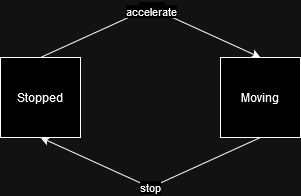
\includegraphics{images/typestate.drawio}
        \caption{Typestate Visualisierung}
        \label{fig:typestate-programming-1}
    \end{figure}

    \note<2>{
        \begin{itemize}
            \item Hier sehen wir das Konzept Visualisiert
            \item Wir haben zwei States: Stopped Moving
            \item Stopped ist der initial-State der mit new() erstellt werden kann
            \item Danach kann mit accelerate und stop\_after kontrolliert zwischen den States gewechselt werden
        \end{itemize}
    }

\end{frame}

\begin{frame}[fragile,t]{Typestate Programming 2}
    State "Stopped" initialisieren:
    \begin{lstlisting}[language=Rust,escapechar=@,label={lst:typestate-programming-2-1}]
let car_state: Stopped = Stopped::new();
println!("Starting at {} m", car_state.get_distance());
\end{lstlisting}
    \codeoutput{code/04-typestate1.txt}

    \note<1>{
        \begin{itemize}
            \item Hier sehen wir wie mit der associatierten Funktion "new" eine instanz von Stopped erstellt wird
            \item Initial hat Stopped immer eine distance von 0, die Distanz kann nur durch den wechsel durch die States angepasst werden
        \end{itemize}
    }

    \pause zu State "Moving" übergehen
    \begin{lstlisting}[language=Rust,escapechar=@,label={lst:typestate-programming-2-2}]
let new_car_state: Moving = car_state.accelerate(
    5, // acceleration in m/s^2
    2 // how long to accelerate in seconds
);
println!("Accelerated to {} m/s", new_car_state.get_velocity());
\end{lstlisting}
    \codeoutput{code/04-typestate2.txt}

    \note<2> {
        \begin{itemize}
            \item Stopped hat die Funktion "accelerate", welche eine Instanz von "Moving" zurückgibt
            \item Dies ist der einzige Weg wie der State "Moving" erreicht werden kann
            \item Moving hat eine geschwindigkeit, die ausgelesen werden kann
        \end{itemize}
    }
\end{frame}



\begin{frame}[fragile,t]{Typestate Programming 3}
    zurück zum State "Stopped"
    \begin{lstlisting}[language=Rust,escapechar=@,label={lst:typestate-programming-3-1}]
let final_car_state: Stopped = new_car_state.stop_after(
    10 // after how many seconds to stop moving
);

println!("Reached destination at {} m", final_car_state.get_distance());
    \end{lstlisting}
    \codeoutput{code/04-typestate3.txt}

    \note{
        \begin{itemize}
            \item Schlussendlich kann mit stop\_after wieder zum State Stopped zurückgekehrt werden
            \item Jetzt hat sich die Distanz erhöht, da für eine gewisse Zeit mit einer gewissen Geschwindigkeit bewegt wurde
            \item Die kann in Rust sehr einfach implementiert werden, da die Typisierung strict ist
            \item Dadurch dass es keine Vererbung gibt, kann auch nicht einfach ein CustomMoving State erstellt werden
        \end{itemize}
    }
\end{frame}

% Tasks & Communication inkl. panic!() :-)

% Patterns & Matching

% Example import from file
\begin{frame}{Fibonacci in rust}
    Fibonacci example

    \mylistingHiglight{22}{31}{Rust}{fibonacci-recursive}{\btLstHL<1>{}\btLstHL<2>{27-29}}{../rust/exercise-prolog-w3-1/src/main.rs}

    \note{
        Still notes
    }
\end{frame}

% Example direct code, note the [fragile] annotation
\begin{frame}[fragile]{Direct filter\_map\_reduce}
    Map and reduce example

    \begin{lstlisting}[language=Rust,escapechar=@,label={lst:map_reduce-test}]
fn filter_map_reduce(list: &[&str]) -> String {
    list.iter()
        .filter(|e| e.starts_with("T"))
        .map(|e| e.to_uppercase())
        .collect::<Vec<String>>().join(" ")
}\end{lstlisting}

    \note{
        Still notes
    }
\end{frame}

% Spawn & Channels

% Cargo: Test & Build
\begin{frame}{Cargo}
    \framesubtitle{Build system and package manager for Rust}
    Cargo kommt mit einigen befehlen, die auch von anderen Build-Tools kennt.
    \codeoutput{code/08-cargo.txt}
    \pause
    Pakete: \url{https://crates.io} Doku: \url{https://docs.rs}\\
    Dependency hinzufügen:
    \codeoutput{code/08-cargo-add.txt}
    \pause
    Konfiguration über \texttt{Cargo.toml} Datei, versionen werden in \texttt{Cargo.lock} festgelegt.
\end{frame}


% Final slides here

\begin{frame}{Related work}
    \framesubtitle{Related work subject \#1}
    \begin{columns}[T]

        \column{0.5\textwidth}
        column left

        \column{0.5\textwidth}
        column right
    \end{columns}

    \note{
        Notes....
    }

\end{frame}

\begin{frame}{Questions and answers}
    \begin{center}
    {\fontsize{40}{50}\selectfont Thank You! \\[10pt] Q \& A}
    \end{center}
\end{frame}

%% REFERENCES
% allowframebreaks: creates multiple slides if it is to long for one
\begin{frame}[allowframebreaks]{References}
    \begin{thebibliography}{}
        \setbeamertemplate{bibliography item}[book]
        \bibitem{DeepLearning}
        Goodfellow, Ian, Yoshua Bengio, and Aaron Courville.
        \newblock \emph{Deep Learning}.
        \newblock MIT Press, 2016.

        \setbeamertemplate{bibliography item}[article]
        \bibitem{FaceNet}
        Schroff, Florian, Dmitry Kalenichenko, and James Philbin.
        \newblock \emph{FaceNet: A Unified Embedding for Face Recognition and Clustering}, 2015.
        \newblock \url{https://arxiv.org/abs/1503.03832}

        \setbeamertemplate{bibliography item}[online]
        \bibitem{DCASE}
        Dekkers, Lauwereins, Thoen et al.
        \newblock \emph{DCASE Challenge 2018 Task 5}, 2018.
        \newblock \url{http://dcase.community/challenge2018/task-monitoring-domestic-activities}
    \end{thebibliography}
\end{frame}


%%
\end{document}
